\newpage
\section{Tropisms} \label{sec::tropism}

The change in root growth direction is described by tropisms. In the following we show how to implement directed growth toward higher water conent or nutrient concentration, and demonstrate how to simply make new user defined tropism rules. 


\subsection{Hydro- and chemotropism} \label{sec:hydro}

Root growth direction is influenced by soil conditions such as water content, soil strength, or nutrient concentration. In the following example we model the influence of a nutrient rhich layer to root system development

\lstinputlisting[language=Python, caption=Example 4a]{../../examples/python/example4a_hydrotropism.py}

\begin{itemize}

\item[6-9] Creates the root system and opens the parameter file

\item[12-17] Change the tropism for all root types: L13 modifies the axial resolution, L14 set the tropism to hydrotropism, and L15-16 sets the two tropism parameters. The parameter $\sigma$ is set to 0.4 for the tap root ($subType$ = 1), and to 1. for the rest of the root types.

\item[19-25] Definition of a static soil property using SDF. We first define the geometry (L20-L21), and then create a static soil (L22) that obtains the maximal value $maxS$ inside the geometry, 
$minS$ outside the geometry, and linear slope with length $slope$. At the boundary the soil has the value $(maxS+minS)/2$.

\item[28] Sets the soil. Must be called before RootSystem::initialize()

\item[41] Initializes the root system, and among others sets up the hydrotropism. 

\item[33-39] Simulation loop

\item[42] Exports the root system geometry

\item[45-46] We actually do not wish to set this geometry, but we abuse the writer of the class RootSytem to export a Python script showing the layer geometry. The resulting ParaView visualization is presented in Figure \ref{fig:chemo}.

\end{itemize}

\begin{figure}
\centering
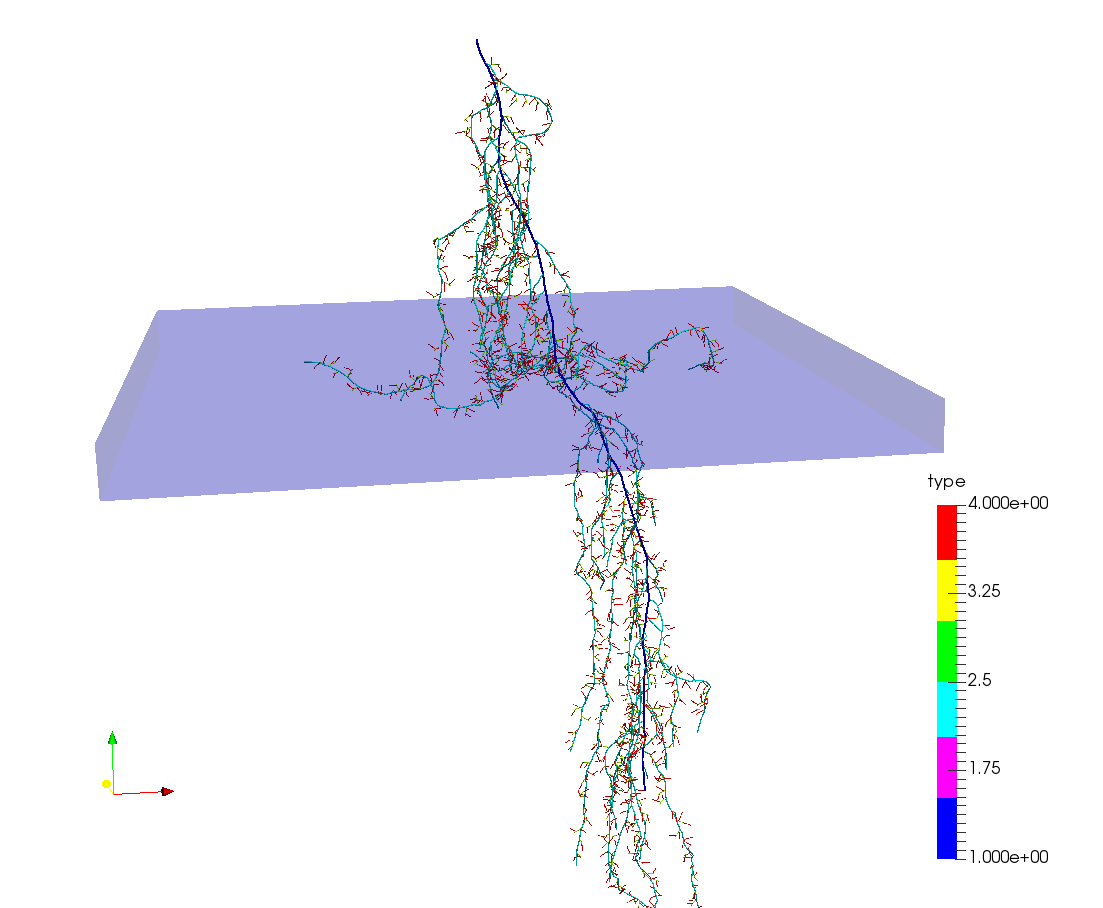
\includegraphics[width=0.7\textwidth]{example4a.png}
\caption{Chemotropism in a nutrient rich layer (Example 4a)} \label{fig:chemo}
\end{figure}



\subsection{Root age dependent growth} \label{sec:usertropism}

Normally, the simulation is created from a set of parameters. For tropisms these are the type of tropism $tt$, number of trials $N$ , and tortuosity $\sigma$. There are only a few predefined tropisms: 'gravi', 'plagio', 'exo', or 'hydro', but it is simple to add user defined tropisms.
The following example demonstrates how to define a root age dependent tropism, where roots first grow according to exotropism (following the inital growth direction), and after a certain age change to gravitropic growth.

The new tropism class must be derived from the class Tropism. In CPlantBox tropism is realised with a random optimization process, where the 'best' direction is chosen from $N$ possible direction, according to an objective function that is minimized. Normally, it is sufficient to overwrite this Tropism::tropismObjective to change the tropsim behaviour. This can be done in Python or in C++. The classes Hydrotropism, Gravitropism, and Plagiotropism (in tropisms.h) are examples for this procedure.

If the whole concept of random optimization is altered, Tropism::getUCHeading must be overwritten, which is only possible in C++. If the geometry model is also changed Tropism::getHeading must be overwritten.

The following example shows how to implement a new tropism in Python. Two new tropism are introduced:
The first does nothing but to output the incoming arguments of the method Tropism::tropismObjective to the command line (e.g. for debugging). The second one root age depenent tropism that starts with exotropism and changes with time to gravitropism depending on the root age.

\lstinputlisting[language=Python, caption=Example 4b]{../../examples/python/example4b_usertropism.py}

\begin{itemize}

\item[8-19] Creates a new tropism that just writes incoming arguments of Tropism: :tropismObjective to the command line. This can be used for debugging. The new class is extended from rb.Tropism, and the method Tropism::tropismObjective is overwritten with the right number of arguments.

\item[22-37] Again, we extend the new class from rb.Tropism. In L25-30 we define our own constructor. Doing this two things are important: (a) the constructor of the super class must be called (L26), and (b) the tropism parameters $n$, and $\sigma$ must be set (L29). 
Furthermore, the constructor defines two tropisms: exo- and gravitropism, that are used in Tropism::tropismObjective at a later point, and a root age that dermines when to switch betwee exo- and gravitropism. \\
In L32-L37 the method Tropism::tropismObjective is defined. We choose the predefined objective function depending on the root age.

\item[41-45] Sets up the simulation.

\item[48-51] L48,L49 creates the first user defined tropsim. Since we did not define a constructor Tropism::setTropismParameter must be called. L50 creates the second user defined tropism.  In L51 the tropism is chosen, using the method Tropism::setTropism. The second argument states for which root type it applies. 
Number 4 is the (default) root type for basal roots, -1 states that the tropism applies for all root types (default = -1).

\item[54-58] The simulation loop. 

\item [61] Exports the result producing Figure (\ref{fig:tropism}). 

\item [64] VTK plot.

\end{itemize}

\begin{figure}
\centering
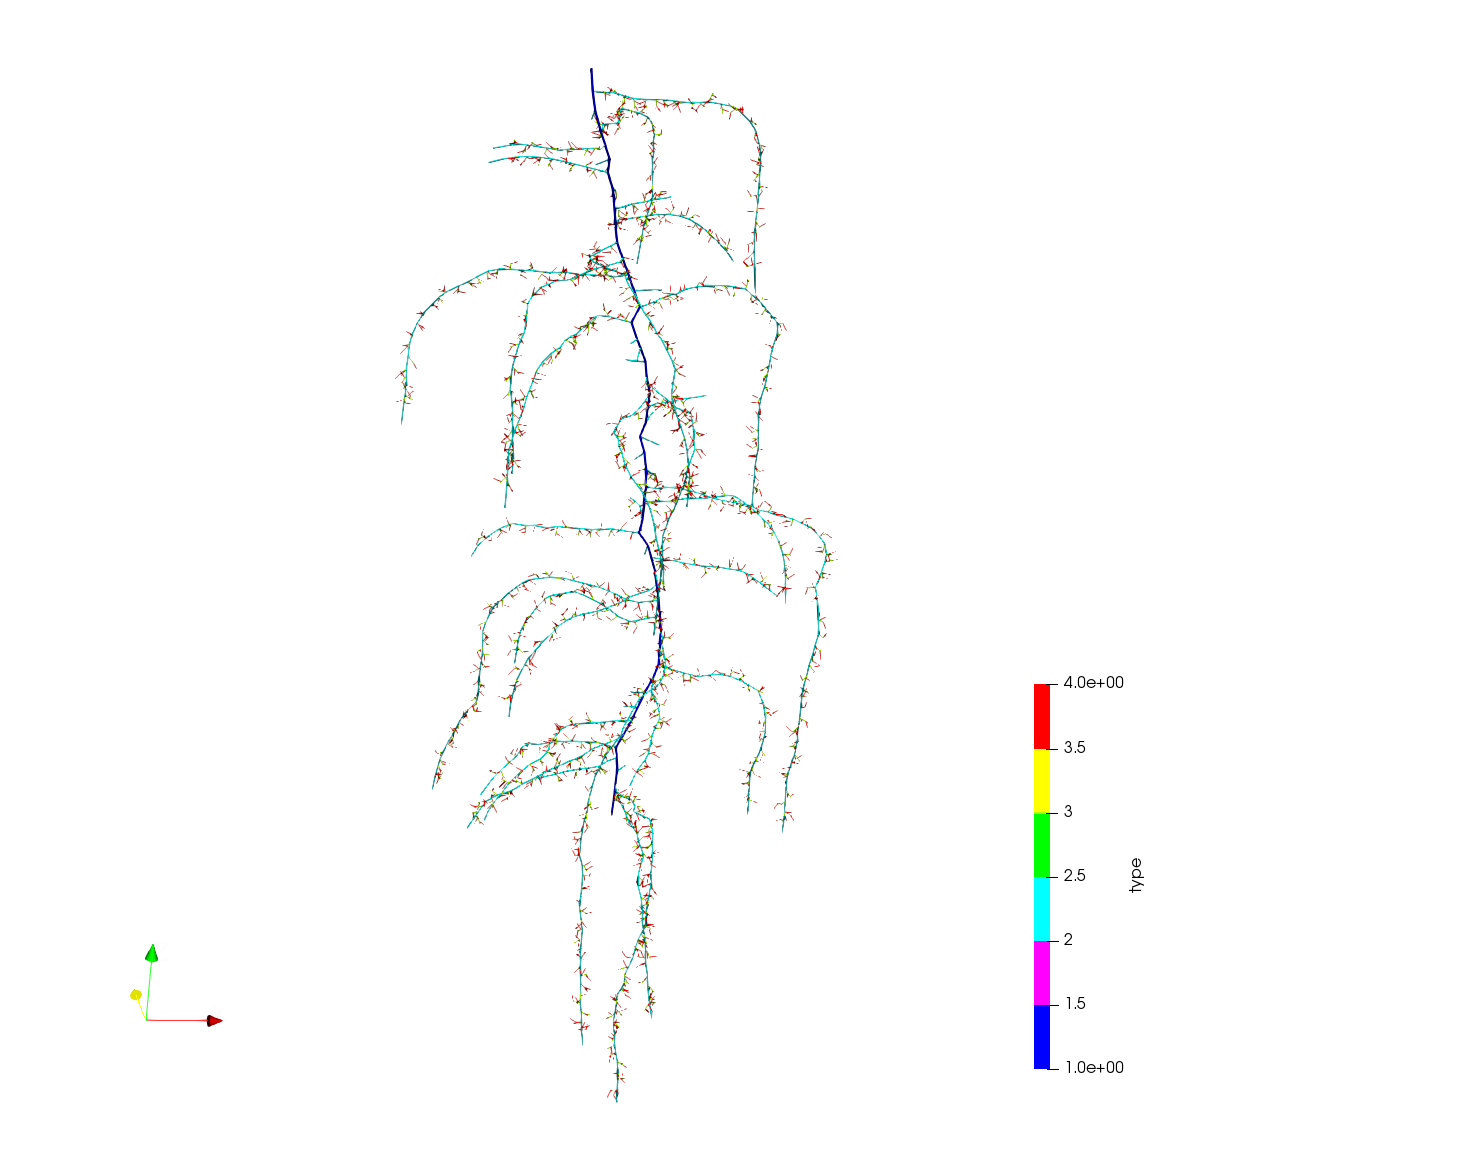
\includegraphics[width=0.7\textwidth]{example4b.png}
\caption{Depending on root age the laterals follow plagio- or gravitropism (Example 4b)} \label{fig:tropism}
\end{figure}

